% Preamble
\providecommand{\main}{../..}
\documentclass[class=article, crop=false]{standalone}

% Packages
\usepackage{\main/packages}
\usepackage{graphicx}
\usepackage{amsmath}

% Configurations
\graphicspath{{\main/images/}{images/}}
\cellspacetoplimit 4pt
\cellspacebottomlimit 4pt

% Document
\begin{document}
    \section{TOPIC 2 - Radiation Integrals}
    In the analysis of radiation problems, the usual procedure is to specify the sources and
    then require the fields radiated by the sources.
    This is in contrast to the synthesis problem where the radiated fields are specified,
    and we are required to determine the sources.
    It is a very common practice in the analysis procedure to introduce auxiliary functions,
    known as \emph{vector potentials}. \\
    The most common vector potential functions are the $A$ (magnetic vector potential) and $F$
    (electric vector potential), also another pair of potential is the \emph{Hertz potentials} $\Pi_e$ and $\Pi_h$.
    \emph{
        Although the electric and magnetic field intensities ($E$ and $H$) represent physically measurable
        quantities, among most engineers the potentials are strictly mathematical tools.
    }
    The introduction of the potentials often simplifies the solution even though it may require
    determination of additional functions. While it is possible to determine the $E$ and $H$
    fields directly from the source-current densities J and M, as shown in Figure\ref{fig:solutionpaths}
    It is usually much simpler to find the auxiliary potential functions first and then determine the $E$ and $H$.
    This two-step procedure is also shown in Figure\ref{fig:solutionpaths}.
    \footnote{
        The above is quoted directly from the textbook\cite{BALANIS}
    }\\

    \begin{figure}[h!]
        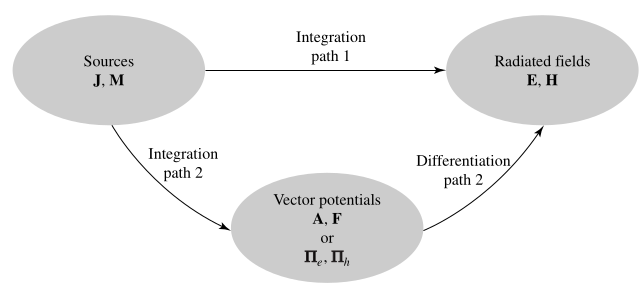
\includegraphics[width=\textwidth]{topics/2/solutionpaths.png}
        \caption{Solution paths for computing fields radiated by sources \cite{BALANIS}}
        \label{fig:solutionpaths}
    \end{figure}

    \newpage

    \subsection{Maxwell's Equations}
    Maxwell's equations constitute the radiation field produced by the sources.\\
    \begin{table}[h]
        \centering
        \begin{tabular}{||c|c|c||}
            \hline
            \textbf{Equation} & \textbf{Differential} & \textbf{Phasor} \\
            \hline\hline
            \emph{Faraday's Law} & $ \curl E = - \pdv{\beta(r, t)}{t} $  & $ E = -j  \omega \beta $  \\
            \emph{Ampere's Law} & $ \curl H = \pdv{D(r,t)}{t} + J(r,t) $ & $ \curl H = j \omega D + J $ \\
            \emph{No Free Magnetic Dipole} &  $ \div B = 0 $ & $ \div B = 0 $ \\
            \emph{Gauss' Law} & $\div D = \rho(r,t) $ & $\div D = \rho $ \\
            \hline
        \end{tabular}
        \caption{Maxwell's equations in differential and phasor forms}
        \label{table:maxwelleqs}
    \end{table}
    \subsection{Procedure to Find Fields for $M$ and $J$ Sources}
    \textbf{Consider the following figure\ref{fig:generalsourceintegral} as a reference to all relevant sections}
    \begin{figure}[h!]
        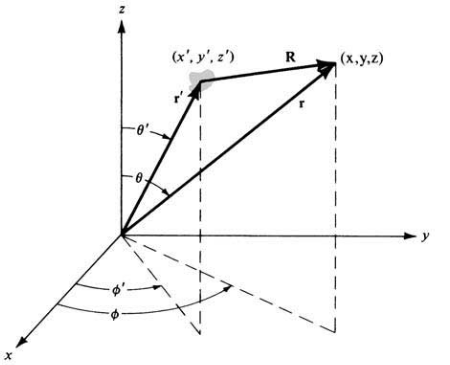
\includegraphics[width=\textwidth]{topics/2/generalsourceintegral.png}
        \caption{General Source radiating a field \cite{BALANIS}}
        \label{fig:generalsourceintegral}
    \end{figure}

    In summary form, the procedure that can be used to find the fields is as follows: \\

    \emph{Summary}: \\

    \begin{enumerate}
        \item Specify $J$ and $M$. (electric and magnetic current density sources)
        \item \begin{enumerate}
                  \item Find $A$ due to $J$ using: \begin{equation}
                             A(r, \phi, \theta) = \frac{\mu}{4 \pi} \iiint_v J \frac{\mathrm{e}^{-jKR}}{R} \dd V
                  \end{equation}
                  \item Find $F$ due $M$ using:  \begin{equation}
                             F(r, \phi, \theta) = \frac{\epsilon}{4 \pi} \iiint_v M \frac{\mathrm{e}^{-jKR}}{R} \dd V
                  \end{equation}
        \end{enumerate}
        \item \begin{enumerate}
                  \item Find $H_A$ and $E_A$ using:
                  \begin{equation}
                                H_A = \frac{1}{\mu} \curl A
                  \end{equation}
                  \begin{equation}
                                E_A = -j \omega A - j \frac{1}{\omega \mu \epsilon} \grad (\div A)
                  \end{equation}
                  \item Find $E_F$ and $H_F$ using:
                  \begin{equation}
                      E_F = - \frac{1}{\epsilon} \curl F
                  \end{equation}
                  \begin{equation}
                      H_F = - j \omega F - \frac{j}{\omega \mu \epsilon} \grad (\div F)
                  \end{equation}
        \end{enumerate}
        \item Total fields are determined by:
        \begin{equation}
            E = E_A + E_F = - j \omega A - j \frac{1}{\omega \mu \epsilon} \grad (\div A) - \frac{1}{\epsilon} \curl F
        \end{equation} or
        \begin{equation}
            E = E_A + E_F = \frac{1}{j \omega \epsilon} \curl H_A - \frac{1}{\epsilon} \curl F
        \end{equation}
        \begin{equation}
            H = H_A + H_F = \frac{1}{\mu} \curl A - j \omega F - j \frac{1}{\omega \mu \epsilon} \grad (\div F)
        \end{equation} or
        \begin{equation}
            H = H_A + H_F = \frac{1}{\mu} \curl A - \frac{1}{j \omega \mu} \curl E_F
        \end{equation}
    \end{enumerate}
    \footnote{
        The above is quoted directly from the textbook\cite{BALANIS}
    }

    \subsection{Far Field Approximation of Fields}
    \textbf{
        Far Field Approximation of Magnetic Vector Potential
    }: \begin{equation}
           A(r, \theta ,\phi) \approx \frac{\mathrm{e}^{-jkr}}{r} A^{0}(\theta, \phi)
    \end{equation} Where,
    \begin{equation}
        A^{0}(\theta, \phi) = \frac{\mu}{4 \pi} \iiint_v J \mathrm{e}^{j k \dot r^\prime } \dd V^\prime
    \end{equation} \\
    \textbf{
        Far Field Approximation of $\curl A$
    }: \begin{equation}
           \curl A = - j k \hat{a_r} \times A
    \end{equation}
    \textbf{
        Far Field Approximation of Electric Field $E$
    }: \begin{equation}
           E = -j \omega ( A_\theta \hat{a_\theta} + A_\phi \hat{a_\phi} )
    \end{equation}
    \begin{equation}
        E^0(\theta, \phi) = E^0_\theta \hat{a_\theta} + E^0_\phi \hat{a_\phi}
    \end{equation}
    \begin{equation}
        E =  \frac{\mathrm{e}^{-jkr}}{r} E^0(\theta, \phi)
    \end{equation}
    \textbf{
        Far Field Approximation of Magnetic Field $H$
    }: \begin{equation}
           H^0(\theta, \phi) = \frac{1}{\eta} \hat{a_r} \times E^0(\theta, \phi)
    \end{equation}
    \begin{equation}
        H = \frac{\mathrm{e}^{-jkr}}{r} H^0(\theta, \phi)
    \end{equation}
    \begin{equation}
        H = \frac{1}{\eta} \hat{a_r} \times E
    \end{equation}

    \subsection{Vector Potential Integral for Different Sources}
    \textbf{
        Volumetric Source
    }
    \begin{equation}
        A(r, \phi, \theta) = \frac{\mu}{4 \pi} \frac{\mathrm{e}^{-jKr}}{r} \iiint_v J_v(r^\prime, \theta^\prime, \phi^\prime)
        \mathrm{e}^{-jKr^\prime} \dd V^\prime
    \end{equation}
    \begin{equation}
        F(r, \phi, \theta) = \frac{\epsilon}{4 \pi} \frac{\mathrm{e}^{-jKr}}{r} \iiint_v
        M_v(r^\prime, \theta^\prime, \phi^\prime) \mathrm{e}^{-jKr^\prime} \dd V^\prime
    \end{equation}
    \textbf{
        Surface Source
    }
    \begin{equation}
        A(r, \phi, \theta) = \frac{\mu}{4 \pi} \frac{\mathrm{e}^{-jKr}}{r} \iint_s J_s(r^\prime, \theta^\prime, \phi^\prime)
        \mathrm{e}^{-jKr^\prime} \dd S^\prime
    \end{equation}
    \begin{equation}
        F(r, \phi, \theta) = \frac{\epsilon}{4 \pi} \frac{\mathrm{e}^{-jKr}}{r} \iint_s
        M_s(r^\prime, \theta^\prime, \phi^\prime) \mathrm{e}^{-jKr^\prime} \dd S^\prime
    \end{equation}
    \textbf{
        Linear Source
    }
    \begin{equation}
        A(r, \phi, \theta) = \frac{\mu}{4 \pi} \frac{\mathrm{e}^{-jKr}}{r} \int_c J_l(r^\prime, \theta^\prime, \phi^\prime)
        \mathrm{e}^{-jKr^\prime} \dd l^\prime
    \end{equation}
    \begin{equation}
        F(r, \phi, \theta) = \frac{\epsilon}{4 \pi} \frac{\mathrm{e}^{-jKr}}{r} \int_c
        M_l(r^\prime, \theta^\prime, \phi^\prime) \mathrm{e}^{-jKr^\prime} \dd l^\prime
    \end{equation}
\end{document}
